\documentclass[a4paper, 11pt]{article}
\usepackage{graphicx}
\usepackage{pdflscape}

\usepackage[left=2cm, text={17cm, 24cm}, top= 3cm]{geometry}
\usepackage[utf8]{inputenc}
\usepackage[czech]{babel}
\title{IDS}
\author{Petr Kaška}
\date{February 2023}

\begin{document}
 
    \begin{titlepage}
        
        \begin{center}
        
            {\Huge\textsc{ Vysoké učení technické v Brně\\
            \huge Fakulta informačních technologií}\\}
            
             \vspace{\stretch{0.382}}
             
             {\LARGE \Huge{1.~Část projektu IDS\\ }}
             
                \vspace{0.5cm}
                
             {\LARGE zadání IUS 37. Rezervace letenek}
               \vspace{\stretch{0.618}}
            
           \end{center} 
            
            {\LARGE 
            {Petr Kaška (xkaska01)\\
            Martin Hemza (xhemza05)}}
            
    \end{titlepage}
    \section{Zadání:}
    \Large{Vaším úkolem je navrhnout webovou aplikaci pro rezervaci letenek. Systém musí uživateli umožnit specifikovat požadavek pomocí místa odletu a příletu, data, času, třídy, letecké společnosti apod. Jedno letadlo může létat na více letech, stejně tak mezi dvěmi destinacemi může létat více letadel různých společností. Zákazník si rezervuje letenku, která může být na několik letů, i různých společností (např. letenka Praha  $\rightarrow$ San Francisco s lety Praha $\rightarrow$ Londýn ČSA, Londýn  $\rightarrow$ San Francisco British Airways). Systém musí umožnit klientovi tisk letového itineráře, který obsahuje informace o dobách příletů a odletů na jednotlivých letištích. Každý typ letadla má různý počet sedadel a jejich rozvržení do tříd. Nemodelujte jednotlivá sedadla. Rezervací může klient zamluvit i více míst v jednom letu. Technická mezipřistání modelovat nemusíte. Systém musí evidovat, která společnost kdy, odkud a kam létá. Cena sedadla v dané třídě může být u každé společnosti jiná, cena letenky je dána součtem cen všech rezervovaných sedadel na všech letech. Pokud klient rezervovanou letenku včas nezaplatí, rezervace se z databáze smaže.}

    \section{Popis:}
        \subsection{ERD:}
        \large{       Tento systém rezervace letenek je rozdělen do osmi entitních množin, jedné generalizace/specializace a jedné slabé entitní množiny, spolu s třemi vazebními vztahy. Existují dva druhy uživatelů: zákazník a cestovní agent. Pro cestovního agenta jsou k dispozici některé atributy, které zákazník nemá, a proto jsme použili generalizaci/specializaci pro cestovního agenta a zákazníka.

Systém obsahuje silnou entitu "lístek", kde každý zákazník může koupit více lístků, ale každý konkrétní lístek je vždy pro jednoho zákazníka. Toto jsme modelovali pomocí vztahu 1:N. Dále je k dispozici silná entitní množina "třída", vazební množina "rozložení sedadel" a silná entitní množina "letadlo", kde instance právě jedné třídy a právě jednoho letadla musí vždy mít stejný počet sedadel. Dále jsme navrhli silnou entitní množinu "aerolinka", protože aerolinky obvykle mají více letadel a víc letů, takže jsme použili vztahy 1:N. Další silnou entitní množinou jsou "let" a "trať". Trasy se obvykle často nemění a létá po nich více letadel různých aerolinií, proto jsme to namodelovali tímto způsobem. Vazební množina "cena třídy" udává cenu jednotlivých lístků v různých třídách jednoho letu.

Slabou entitní množinou, kterou jsme použili, je "letový plán", který závisí na konkrétním letu a je spojena ternárním vztahem s třídou a lístky. Tento přístup nám umožňuje zaznamenat počet sedadel pro konkrétní lístek a ve které třídě jsou sedadla rezervována.}
        
        \subsection{Use Case:}
         \large{Systém se skládá ze 3 aktérů zákazníka, cestovního agenta a administrátora. U zákazníka jsme použili include. Abychom zdůraznily změnu stav letenky na koupená/rezervovaná při interakci s nimi.}
        
  
    \begin{landscape}
    
        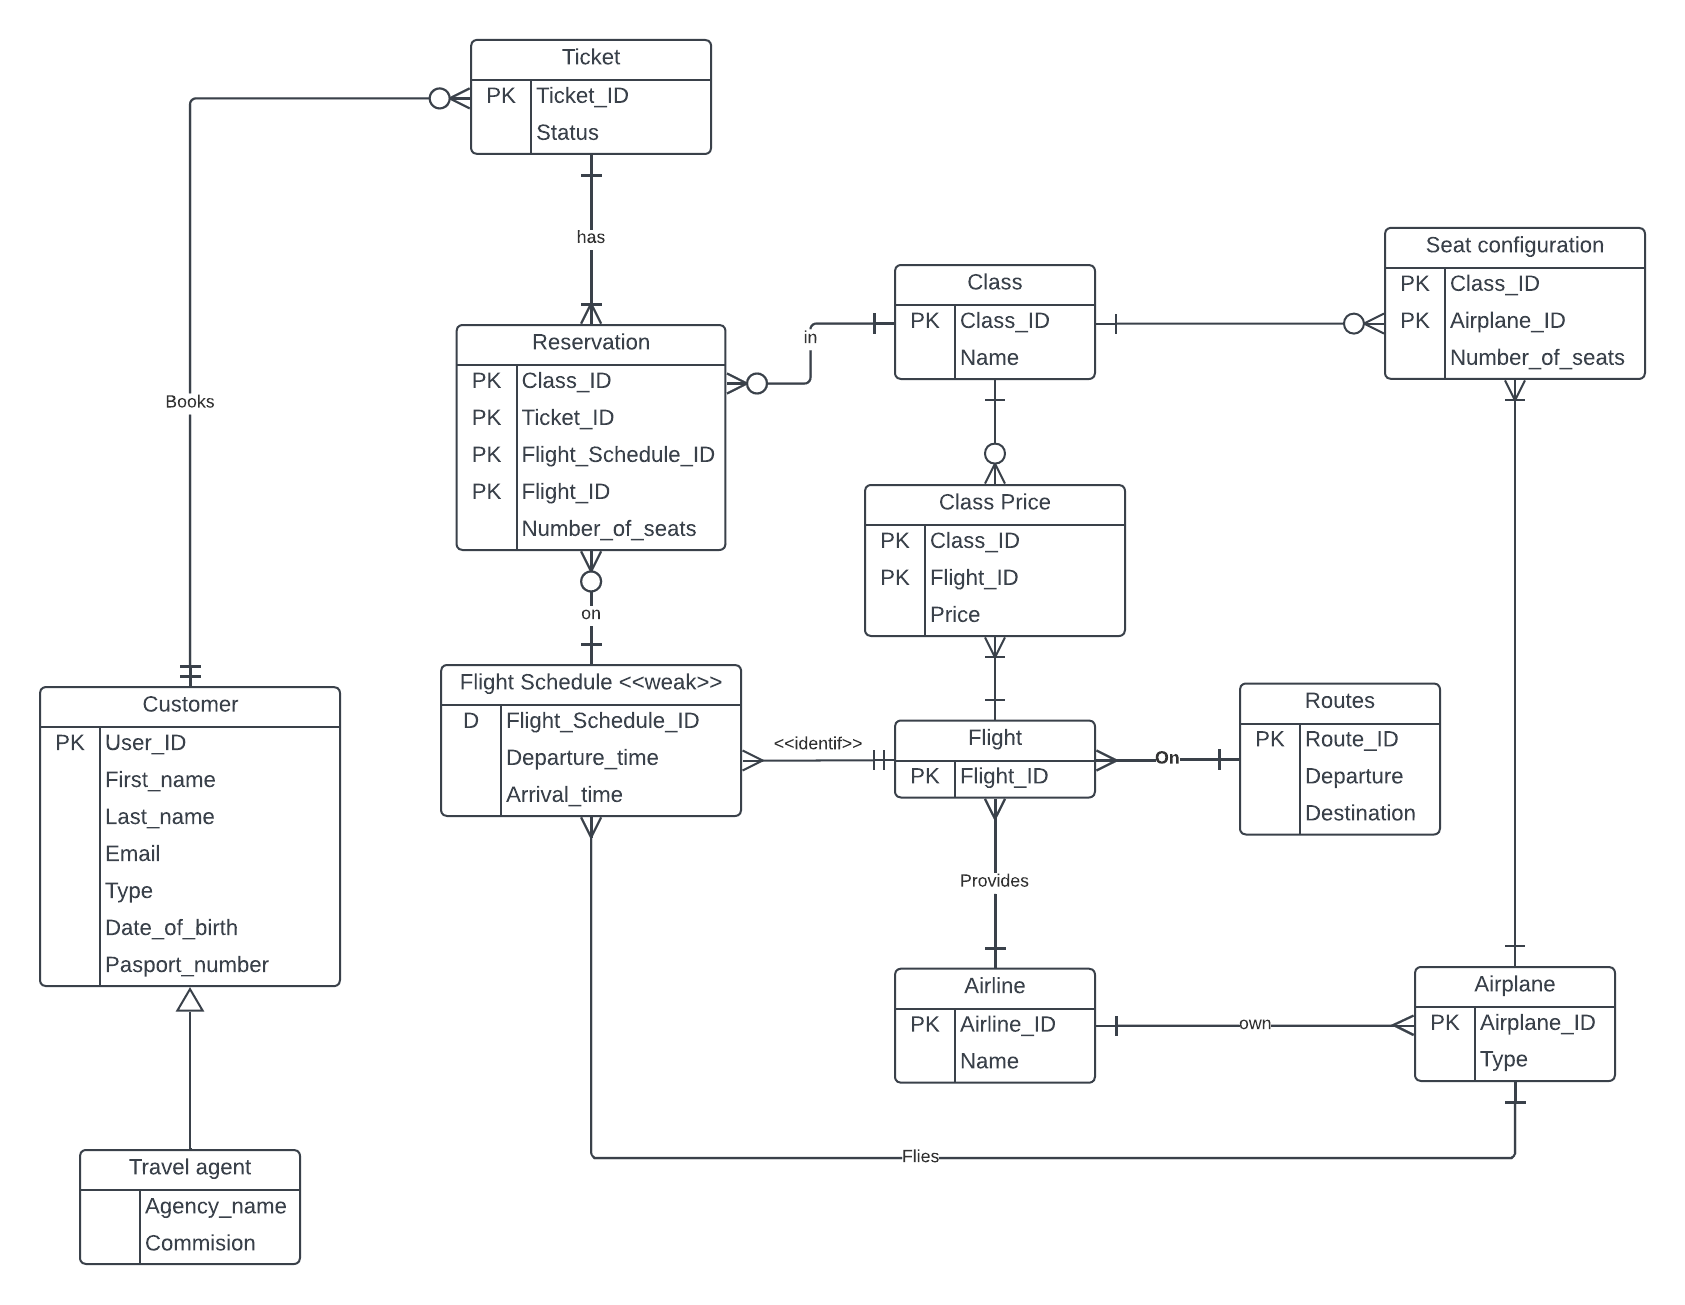
\includegraphics[scale=0.8]{ERD.png}

    \end{landscape}
   
    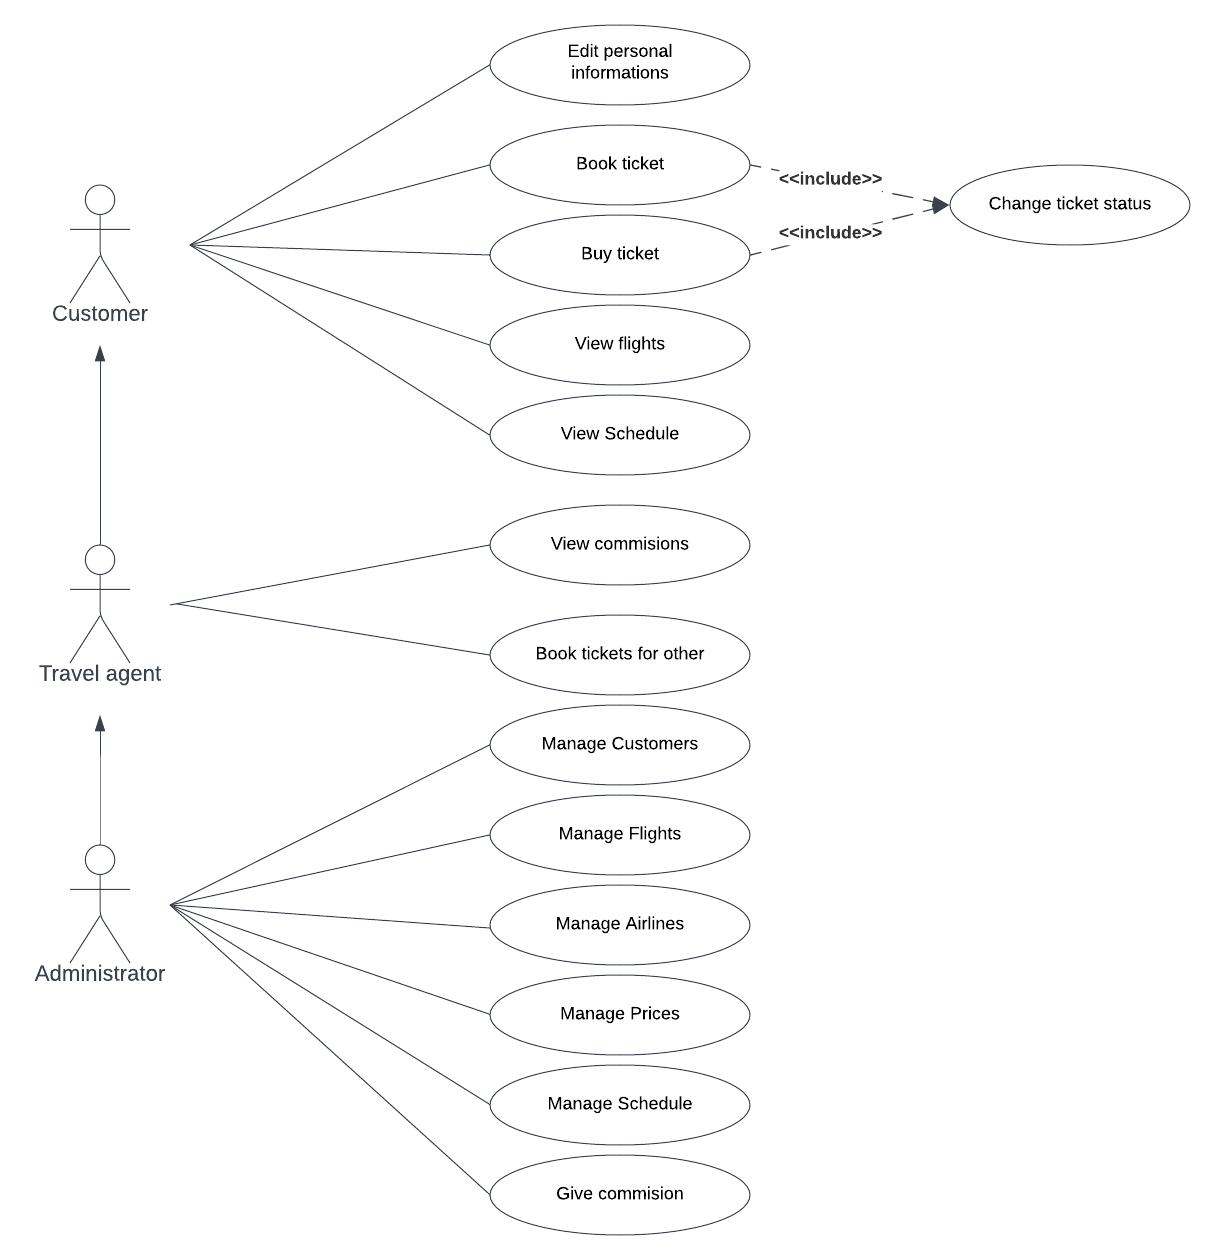
\includegraphics[scale=0.85]{USECASE.png}

\end{document}
